\section{Régularisation et sur-apprentissage}

\subsection{Le sur-apprentissage}
\label{surappsec}

Le \textbf{danger principal} de tout algorithme d'apprentissage automatique est le \textit{sur-apprentissage}. Comme vu dans l'introduction de cette partie, un algorithme d'apprentissage automatique cherche à approximer une fonction capable d'expliquer les données \textbf{et} capable de généralisation. Mais que signifie "généralisation" ?\\

\begin{figure}
    \centering
    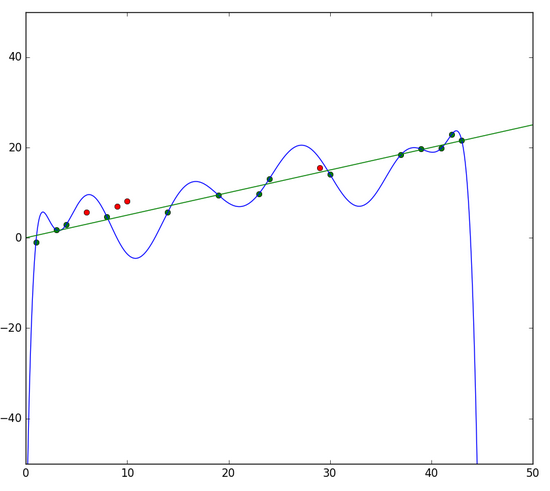
\includegraphics[scale=0.4]{./tex/regularisation/surapp.png}
    \caption{Exemple de sur-apprentissage (bleu) et d'apprentissage optimal (vert)}
    \label{surapp}
\end{figure}

\noindent Pour expliquer cette problématique, observons la Figure \ref{surapp}. Nous pouvons observer des points verts représentant les données du jeu d'apprentissage et des points rouges, les données inconnues qui doivent être prédites par le modèle. La courbe bleu et la courbe verte présentent deux fonctions apprises par deux modèles. On peut apercevoir que la courbe bleue passe par l'ensemble des points verts alors que la courbe verte possède une moins bonne performance. On peut donc naïvement dire que la courbe bleue a mieux appris. C'est vrai dans l'absolu: la courbe bleue a mieux appris le jeu de données d'apprentissage mais en plus d'apprendre le comportement général des données, elle a appris son bruit, ce qui lui donne son comportement oscillant et "imprévisible". Le fait d'apprendre le bruit est appelé \textit{sur-apprentissage} et est désastreux pour le modèle qui perd ainsi sa capacité de généralisation. Au contraire, la courbe verte n'apprend pas le bruit des données. Elle apprend moins les données d'apprentissage mais conserve sa capacité de généralisation. L'idéal est donc de trouver un compromis entre apprentissage du jeu de données et capacité de généralisation: ceci est appelé \textit{compromis biais-variance}.\\

\noindent Une explication graphique est visible sur la Figure \ref{compbv}. Le biais représente l'erreur réalisée sur l'apprentissage des données. Ainsi, un biais très faible sous-entend un sur-apprentissage car le bruit aura été appris. Au contraire, la variance représente l'importance des variations de la fonction hypothèse approximée, i.e la sensibilité du modèle aux variations des données et donc au bruit. De ce fait, plus la variance est élevée, plus le modèle perd en généralisation et devient inutilisable. Et, comme observé sur la Figure \ref{surapp}, le sur-apprentissage favorise un comportement à forte variance (représenté par les oscillations). L'objectif est donc de réaliser un compromis: optimiser la diminution du biais et de la variance.\\

\noindent D'un point de vue expérimental, la notion de biais et de variance est représentée par l'erreur de prédiction réalisée sur l'ensemble d'apprentissage et de test. Ainsi, l'objectif est d'arrêter l'apprentissage lorsque la courbe de prédiction du jeu de test augmente de manière significative alors que la prédiction sur le jeu d'apprentissage tend à diminuer.\\

\begin{figure}
    \begin{tabular}{cc}
        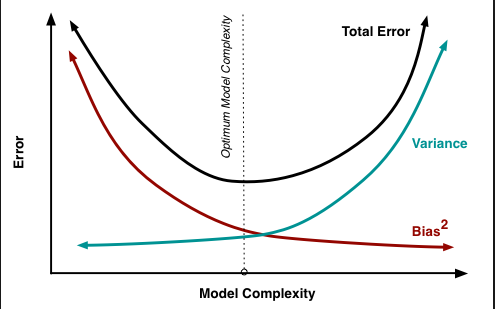
\includegraphics[scale=0.4]{./tex/regularisation/combv.png} & 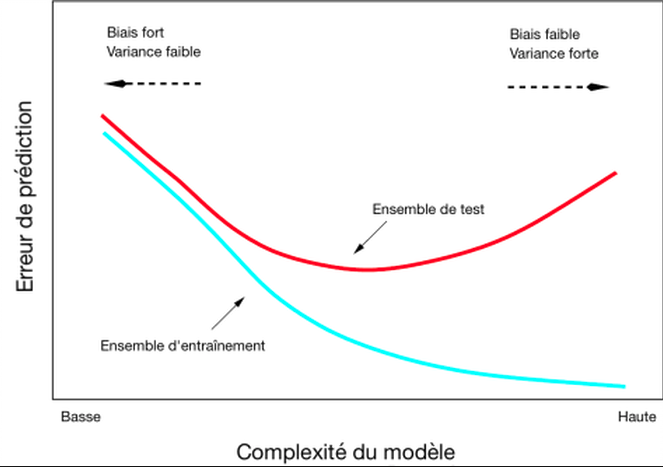
\includegraphics[scale=0.25]{./tex/regularisation/compbv2.png} \\
    \end{tabular}
        \caption{Compromis biais-variance et impact sur le modèle}
    \label{compbv}
\end{figure}

\noindent Bien sur, la problématique du sous-apprentissage existe aussi et représente un modèle trop généraliste qui n'explique pas suffisamment les données d'apprentissage qui discriminent ses prédictions. Un exemple est visible sur la Figure \ref{sousapp} où la fonction crée est bien trop "neutre". Il est évident qu'un modèle sous-entraîné possède des performances faibles.

\begin{figure}
    \centering
    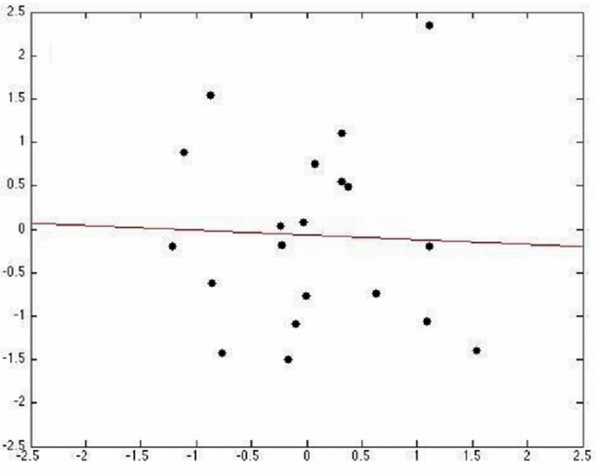
\includegraphics[scale=0.3]{./tex/regularisation/sousapp.png}
    \caption{Exemple de sous-apprentissage}
    \label{sousapp}
\end{figure}

\subsection{Limiter le sur-apprentissage}

\textbf{Important}: Cette partie est fondamentale et doit être comprise pour développer un réseau de qualité, notamment dans le cadre d'architecture très profonde que nous étudierons par la suite.\\

\subsection{Régularisation}
\label{regsec}

Les poids d'un neurone ne sont pas bornés\footnote{Dans les cas d'une architecture standard}. Cette spécificité permet une grande disparité entre les valeurs que peuvent prendre les poids d'un neurone au risque de voir certains poids \textit{exploser} alors que d'autres seraient \textit{faibles}\footnote{Cette particularité est aggravée si les données en entrée du neurone ne sont pas normalisée. Les données d'apprentissage peuvent être normalisées en entrée tout en provoquant ce phénomène en interne.}. Cette différence de valeur est très préjudiciable et favorise un comportement de sur-apprentissage où un neurone sur-réagit aux stimulations portées par les poids de haute intensité. Pour limiter l'explosion des poids, une régulation peut être imposée. \\

\noindent Cette régulation peut être associée à la fonction de coût, lui rajoutant un nouveau critère de discrimination. Ainsi, supposons la fonction de coût définie par Mean Squared Error\footnote{Voir la section \ref{fn_cout} pour plus d'informations}. Elle est définie par: $\boldsymbol{\mathcal{L}}=\frac{1}{n}\sum_{i=1}^{n}(y^{(i)}-\hat{y}^{(i)})^{2}$. Avec une régulation, nous obtenons $\boldsymbol{\mathcal{L}_{reg}}=\frac{1}{n}\sum_{i=1}^{n}(y^{(i)}-\hat{y}^{(i)})^{2}+\boldsymbol{\epsilon(\omega)}$ ou $\epsilon$ dépend uniquement des poids des neurones du réseau. Ainsi, la fonction de coût sera directement dépendant des poids des neurones et tendra à limiter leurs évolutions divergentes.\\

\subsubsection{L1-Régulation}

La première régulation est la L1-Régulation. Elle s'exprime sous la forme $\lambda|\omega|$ où $\lambda$ correspond à l'intensité associée à la régulation. Plus $\lambda$ est élevé, plus on pondère l'importance d'avoir des poids faibles. Ainsi, dans le cas de Mean Squared Error, nous obtenons $\boldsymbol{\mathcal{L}_{reg}}=\frac{1}{n}\sum_{i=1}^{n}(y^{(i)}-\hat{y}^{(i)})^{2}+\lambda|\omega|$. \\

\noindent Cette régulation est très utile dans le cas d'extraction de \textit{feature}. En effet, cette régulation tend à rendre le réseau \textit{sparse} en permettant que des poids deviennent très proches de zéro (annulant ainsi une entrée du neurone). Cette régulation favorise les entrées discriminantes et limite les entrées porteuses de bruit. Il est ainsi possible d'extraire les composantes principales du réseaux. Néanmoins, dans les faits, elle est rarement utilisée car présente de moins bons résultats que la régulation L2 (sauf dans le cas spécifique d'extraction de feature). De plus, n'étant pas quadratique, sa minimisation est difficile.

\subsubsection{L2-Régulation}
\label{l2_reg}
L2-Regulation est définie par la contrainte $\frac{1}{2}\lambda\omega^2$. La fonction de coût régulée devient donc $\boldsymbol{\mathcal{L}_{reg}}=\frac{1}{n}\sum_{i=1}^{n}(y^{(i)}-\hat{y}^{(i)})^{2}+\frac{1}{2}\lambda\omega^2$.\\

\noindent Cette régulation favorise des valeurs de poids proches en limitant les pics de valeurs. Ainsi, elle permet de faire en sorte que le neurone ne se focalise pas sur des entrées dominantes tout en délaissant les autres jugées moins pertinentes. Elle limite dons la sur-spécialisation et de ce fait, l'overfitting. Cette régulation est efficace et très utilisée aujourd'hui.

\subsubsection{ElasticNet-Régulation}

ElasticNet-Régulation est une combinaison linéaire de la Régulation L1 et L2. Elle s'exprime sous la forme $\lambda_1|\omega|+\frac{1}{2}\lambda_2\omega^2$ où $\lambda_1$ et $\lambda_2$ définissent l'importance de cette régulation dans le calcul de la performance du modèle et la pondération entre les deux régulations (comportement équilibré ou pondération d'une des deux régulations). Ainsi, la fonction de coût est dorénavant définie par la relation suivant:  $\boldsymbol{\mathcal{L}_{reg}}=\frac{1}{n}\sum_{i=1}^{n}(y^{(i)}-\hat{y}^{(i)})^{2}+\lambda_1|\omega|+\frac{1}{2}\lambda_2\omega^2$\\

\noindent Cette régulation réunit \textit{le meilleur des deux mondes} (issus de L1 et L2) bien que moins souvent appliquée que la L2-Régulation.

\subsection{Max norm constraints}

Contrairement à la régulation L1 et L2, Max norm constraints ne s'applique pas à la fonction de coût mais directement au vecteur de poids du neurone. Alors que L1 et L2 pénalisent les poids élevés\footnote{Pénaliser augmente la fonction de coût mais il n'y a pas de contrainte directe imposée à l'intégralité du réseau. Ainsi, L1/L2 favoriseront la limitation des poids les plus élevées en priorité alors que Max norm constraints les corrigera tous sans distinction}, Max norm constraints agit directement sur ces derniers. Ainsi, chaque vecteur de poids doit respecter la condition $||\omega||_2 < cnst$ ou cnst de petite taille (2,3 voire 4 par exemple). Si l'égalité n'est pas respectée, l'intégralité des poids est normalisée\footnote{Ce n'est pas la normalisation au sens statistiques !} afin de respecter la condition.\\

\noindent Cette régulatisation est particulièrement performante associée avec le \textit{DropOut}\footnote{Voir http://www.cs.toronto.edu/~rsalakhu/papers/srivastava14a.pdf, partie 5.1} mais présente la difficulté de paramétrage du seuil (cnst) qui est un hyperparamètres. Sa détermination se fait de manière empirique et expérimentale, ce qui peut rendre sa recherche délicate.

\subsection{DropOut}

Contrairement à la régulation qui agit sur les neurones de manière isolée, le DropOut\cite{dropout_deep} est une approche de régulation d'architecture, i.e une approche qui influence l'interaction entre neurones. Le DropOut sélectionne aléatoirement (selon une probabilité $\rho$) des neurones du réseau et leur impose une activation\footnote{L'activation correspond à la somme pondérée des entrées} nulle. La sélection des neurones inactifs est renouvelée à chaque donnée d'apprentissage. Lors de l'utilisation du réseau hors apprentissage, chaque sorties des neurones concernées par le DropOut sont multipliées par $\rho$ et toutes sont actives. Un exemple est visible sur la Figure \ref{dropoutdropco}.\\

\noindent Cette méthode permet de limiter l'inter-dépendance (Voir Section \ref{dead_relu}) entre les neurones et favorise la création d'un réseau éparse. L'apprentissage du modèle est ainsi plus robuste, plus rapide et moins soumis aux problématiques associées au gradient. Le DropOut est souvent exploité en plus d'une \textit{Régulation} des poids bien que son comportement soit comparable à la régulation L2. Une valeur standard pour $\rho$ est 0.5. Cette approche est souvent employée pour les réseaux Full-Connected mais peut être appliquée à d'autres architecture notamment les réseaux convolutifs. Néanmoins, l'efficacité de son utilisation sur des couches convolutives est sujet à débat.\\

\noindent \textbf{Important}: DropOut est souvent utilisé avec des fonctions d'activation f tel f(0)=0. En effet, le DropOut ne force pas la sortie à 0 mais son activation. Ainsi, si une fonction d'activation n'est pas nulle en 0, le neurone ne sera pas (complètement) inactif bien que son comportement soit constant. De plus, le biais est indépendant de l'activation et n'est pas soumis au DropOut.

\begin{figure}
\centering
        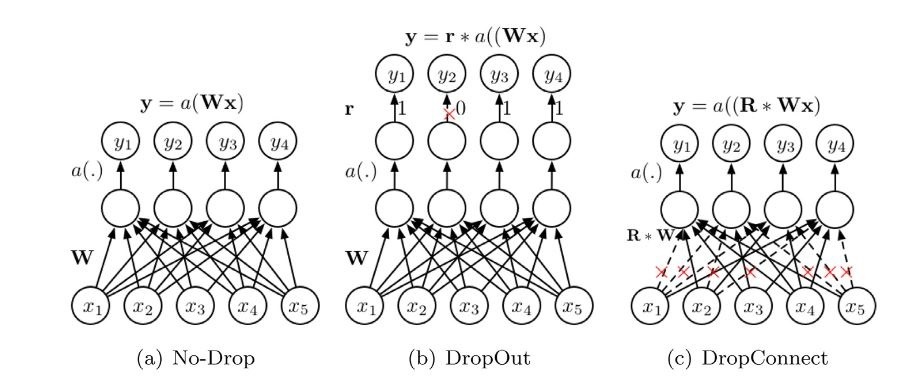
\includegraphics[scale=0.4]{./tex/regularisation/droppic.png}
    \caption{Comparaison d'un réseau sous DropOut et DropConnect}
    \label{dropoutdropco}
\end{figure}

\begin{figure}
   \centering
         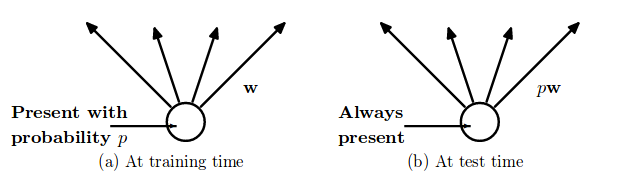
\includegraphics[scale=0.4]{./tex/regularisation/drop2.png} \\
    \caption{Relation des poids après DropOut}
    \label{dropout_fig}
\end{figure}

\subsection{DropConnect}

\noindent DropConnect\cite{dropconnect_deep} est une généralisation de DropOut. Au lieu de supprimer l'activité d'un neurone en bloquant son activation, cette méthode annule les poids d'entrée du neurone de manière indépendante selon une probabilité $\rho$. Ainsi, un neurone peut voir son activation éteinte (comparable à DropOut) ou juste partiellement. Un exemple de DropConnect est visible sur la Figure \ref{dropoutdropco}. Cette méthode est moins utilisée que DropOut et ses résultats plus rares. Il n'est pas aisé de déterminer quelle approche est la plus performante objectivement mais le DropConnect offre plus de souplesse et de configurations possibles.

\subsection{DisturbLabel}

\noindent DisturbLabel\cite{disturblabel} est une méthode de régularisation qui exploite l'approche par \textit{bruitage}. L'idée derrière cette méthode est de modifier aléatoirement le label d'une donnée d'apprentissage dans chaque minibatch d'apprentissage. On suppose une problématique multi-classe bien qu'il soit possible de généraliser à une problématique multi-label.\\

\noindent Ainsi, DisturbLabel rajoute une étape de sampling supplémentaire qui génère, pour chaque couple de donnée $(x_D,y_C)$, un vecteur label $\Hat{y}=[\Hat{y}_1,..., \Hat{y}_C]$ (avec C, nombre de label) issu d'une loi Multinouilli (Bernouilli généralisée) $P(\alpha)$ tel que:
\begin{align*}
    \Hat{c} &\sim P(\alpha)\\
    \Hat{y}_c &= 1\\
    \Hat{y}_i &= 0, \ \forall i \neq \Hat{c}\\
\end{align*}

\noindent De même, $P(\alpha)$ est définie par $p_c=1-\frac{C-1}{C}$ et $p_i=\frac{1}{C}*\alpha$ pour tout $i \neq c$ et c, indice du label valide. $\alpha$ est le \textit{taux de bruitage}. Si $\alpha=0$, il n'y a pas de bruitage. Si $\alpha \rightarrow 100\%$, alors la labellisation du jeu d'apprentissage est aléatoire. Il est donc nécessaire de garder un $\alpha$ de faible valeur.

\subsection{Dense-Sparse-Dense training}

Le Dense-Sparse-Dense\cite{dsd_deep} training est une méthode comparable à une variante du DropOut/DropConnect. Cette méthode cherche à proposer une méthode d'apprentissage plus efficace dans le cadre de réseaux très profonds. L'idée soutenue par cette méthode est qu'un réseau très profond est capable d'acquérir une compréhension plus profonde d'un phénomène mais plus enclin à en apprendre le bruit et le comportement instable. Leur postulat est que le bruit est porté par les poids faibles des neurones. Ainsi, l'objectif est d'être capable d'isoler les poids d'importance qui propagent une information fiable et les poids qui propagent le bruit. Pour cela, cette méthode (Figure \ref{dsd_fig}) se découpe en 3 phases:

\begin{enumerate}
    \item \textbf{Initial Dense Phase}: L'apprentissage du réseau est fait normalement sans contrainte particulière. Les méthodes de régulations (et autres) peuvent être exploitées durant cette phase. L'objectif de cette phase n'est pas "d'apprendre" mais de détecter les poids influents et non influents (en fonction de leurs valeurs absolues).

    \item \textbf{Sparse Phase}: Durant cette phase, les poids sont classées par couche selon leurs valeurs. Seuls les $\lambda$\% plus élevés sont conservés intacts, les autres devenant nuls. $\lambda$ est un hyperparamètre à déterminer (il est conseillé de prendre une valeur entre 25\% et 50\% comme valeur par défaut). Le réseau devient alors éparse, permettant d'obtenir un réseau plus robuste et plus économe. Il est empiriquement montré qu'un réseau éparse tend à avoir des résultats équivalents voir meilleurs qu'un réseau dense car ce dernier est plus sensible aux problématiques d'apprentissage. Un apprentissage du réseau est réalisé avec cette architecture.

    \item  \textbf{Final Dense Phase}: Durant cette phase, les connexions coupées sont restaurées. Les poids restaurés sont initiés à 0 et le pas d'apprentissage du gradient faible (1/10 du pas initial). En effet, le réseau actuel présente une stabilité et une convergence correcte. Il n'est donc pas souhaitable de "bouleverser" son architecture mais juste de favoriser sa performance en finalisant son comportement dans ses détails d'apprentissage. Le réseau peut ainsi converger vers un meilleur minimum local voire "en sortir" vers un autre selon le cas.

    \item \textbf{Répétition}: Ce cycle (3 phases) peut être répété afin de favoriser une meilleure convergence.
\end{enumerate}

\begin{figure}
    \centering
    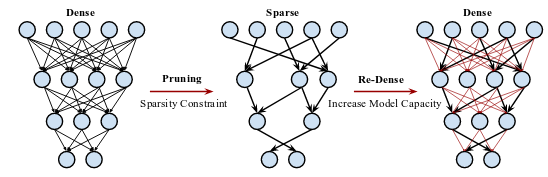
\includegraphics[scale=0.4]{./tex/regularisation/dsd.png}
    \caption{Dense-Sparse-Dense Routine}
    \label{dsd_fig}
\end{figure}

\subsection{Batch Normalization}

Batch Normalization\cite{batchnorm_deep} est une méthode qui vise à augmenter la robustesse du modèle en favorisant sa capacité de généralisation. Supposons un jeu de données d'image de chiens blancs, si une image d'un chien noir apparaît lors de la prédiction, il est évident que le réseau ne fonctionnera pas car la distribution des données d'apprentissage et de prédiction ne correspondent pas. Néanmoins, le comportement des données peut être similaire et donc, la fonction obtenue sur les chiens blancs pourraient être effective. Batch Normalization permet d'aligner les distributions et de limiter cette problématique. Un exemple illustratif est visible sur la Figure \ref{bnex}. La justification de performance de cette approche est très mathématique et repose sur un socle solide de Statistiques. Nous ne l'étudierons pas dans cette introduction.\\

\noindent L'idée de Batch Normalization est de généraliser la normalisation des données à travers le réseau de neurones. La méthode est comparable à une normalisation standard mais présente des spécificités associées à la présence d'un minibatch qui représente un sous-ensemble du jeu d'apprentissage (qui plus est, variable). La normalisation réalisée est visible sur la Figure \ref{batchnorm_fig}. Veuillez vous référer à la publication associée\cite{batchnorm_deep} pour plus de détails mathématiques sur son fonctionnement.  \\

\noindent De plus, cette méthode permet de mieux isoler les couches entre elles, limitant l'inter-dépendance, permet d'utiliser un pas d'apprentissage plus important car les données internes au réseau sont normalisées (ce qui limite les valeurs extrêmes et donc les valeurs du gradient) et possède une action de régulation. L'utiliser avec DropOut (ou équivalent) est efficace bien qu'il soit préférable d'utiliser une probabilité plus faible d'éteindre un neurone dans cette configuration. Un gain de vitesse est aussi observé du fait de la limitation des valeurs des données, ce qui favorise une implémentation optimisée.\\

\noindent De même que le DropOut, Batch Normalization fait partie des améliorations majeures proposées dans le cadre du développement d'un réseau de neurones et son utilisation est quasi-récurrente à tout réseau d'ampleur.

\begin{figure}
    \centering
    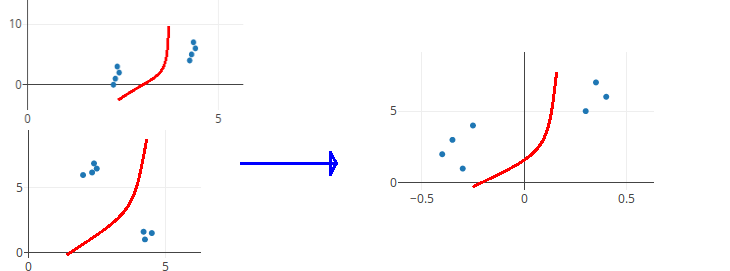
\includegraphics[scale=0.4]{./tex/regularisation/bn1.png}
    \caption{Non-alignement des distributions}
    \label{bnex}
\end{figure}

\begin{figure}
    \centering
 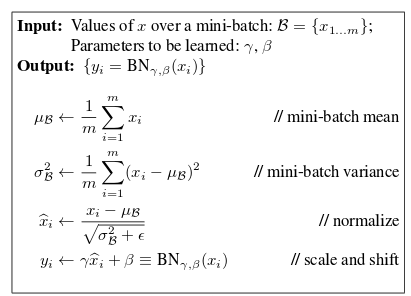
\includegraphics[scale=0.4]{./tex/regularisation/batchnorm.png}
    \caption{Normalisation par Batch Normalization}
    \label{batchnorm_fig}
\end{figure}

\subsection{Critère d'arrêt de l'apprentissage}
Pour réaliser un bon apprentissage, il est nécessaire de considérer le \textit{compromis biais-variance} afin de limiter le sur-apprentissage. Bien que la problématique soit facilement assimilable, s'en prémunir reste difficile.\\

\noindent Une bonne pratique repose sur l'utilisation d'architectures de régulation qui tend à limiter le phénomène de sur-apprentissage\footnote{Phénomène présent lorsque la courbe de biais diminue et la courbe de variance augmente}. Bien que fonctionnelles, ces architectures ne garantissent pas un apprentissage contrôlé. Une approche complémentaire est donc de savoir \textbf{quand} arrêter l'apprentissage afin d'obtenir le meilleur état du modèle. Dans le cas idéal, l'arrêt se situe à l'intersection de la courbe de biais et de variance. Mais comment savoir si on se situe dans un intervalle proche de ce point de référence ?\\

\noindent La courbe de biais est associée aux erreurs de prédiction sur les données d'apprentissage alors que pour la courbe de variance, ce sont les erreurs de prédiction sur les données de validation (Figure \ref{compbv}). La courbe de biais décroît logiquement durant l'apprentissage jusqu'à atteindre une valeur asymptotique caractérisée par un résidu de bruit. Au contraire, la courbe de variance va décroître progressivement avant de croître lorsque le modèle commence à perdre sa capacité de généralisation. L'objectif étant d'assurer la meilleure performance prédictive tout en ayant une forte capacité d'abstraction, se concentrer sur le comportement de la courbe de variance semble prioritaire. Il est ainsi nécessaire de détecter le minimum global de cette fonction alors que la courbe de biais ne présente qu'une importance secondaire. Il serait même dangereux de se concentrer sur la courbe d'apprentissage car une erreur très faible d'apprentissage est souvent associée à un sur-apprentissage important.\\

\noindent Sur la Figure \ref{compbv}, la courbe de variance est idéalisée. Dans les faits, elle présente souvent du bruits et des oscillations locales qui rendent son étude délicate (Figure \ref{early_courbe}). La problématique du minimum local est au coeur du problème et il n'existe pas de solution idéale actuellement pour garantir un arrêt optimal de l'apprentissage du modèle. Néanmoins, plusieurs approches existent et présentent des résultats satisfaisants. Ces fonctions de régulation sont appelées \textbf{Early Stopping}.

\begin{figure}
    \begin{tabular}{cc}
       a) 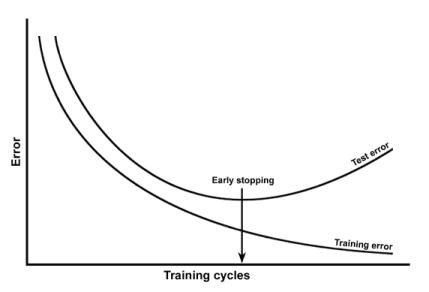
\includegraphics[scale=0.9]{./tex/regularisation/valid_ideal.png} &
         b) 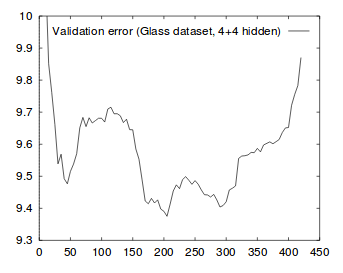
\includegraphics[scale=0.4]{./tex/regularisation/val_reel.png}\\
    \end{tabular}
    \caption{a) Early Stop théorique b) Comportement-type de l'erreur de validation en situation réelle}
    \label{early_courbe}
\end{figure}

\subsubsection{Early Stopping}
Les méthodes \textit{Early Stopping} repose sur la valeur de l'erreur de validation. De ce fait, nous définissons $E_{opt}(t)$, l'erreur de validation la plus faible jusqu'à l'instant t, définie par: $E_{opt}(t)=\underset{t' \leq t}{min}(E_{va}(t'))$ avec $E_{va}$, erreur de validation.

\paragraph{Generalization Loss ($GL_\alpha$)}
La première méthode, nommée Generalization Loss ($GL_\alpha$)\cite{earlystop}, repose sur l'augmentation relative de l'erreur à l'instant t par rapport à $E_{opt}(t)$. Ainsi, si l'augmentation est supérieure à une valeur donnée, l'apprentissage est stoppé. Ce critère examine la tendance absolue de l'évolution de l'erreur de validation et néglige la tendance évolutive locale.\\

\noindent Pour formaliser mathématiquement ce comportement, nous définissons l'erreur (en pourcentage) par:
$$GL(t)=100*(\frac{E_{va}(t)}{E_{opt}(t)}-1)$$
$$Stop: \ GL(t) > \alpha$$

\noindent Cette approche est peu efficace pour lutter contre les minimum locaux. Exploiter ce critère d'arrêt aura tendance à stopper l'apprentissage lorsqu'un minimum local aura été observé. Bien qu'efficace en cas de comportement convexe de la fonction d'erreur, elle est peu performante dans le cas contraire. Expérimentalement, ce critère limitera la capacité d'exploration du réseau durant sa phase d'apprentissage et peut favoriser un arrêt prématuré.

\paragraph{Quotient of Generalization Loss and Progress ($PQ_{alpha}$)}
La méthode $GL_{\alpha}$ ignore le comportement du modèle sur les données d'apprentissage. En ignorant ces informations, ce critère n'a pas connaissance de la situation d'apprentissage du réseau. La variation de l'erreur d'apprentissage peut donc être faible ou élevée sans qu'elle n'ait d'impact sur le critère d'arrêt. Expérimentalement, on observe que le sur-apprentissage arrive souvent lorsque l'erreur d'apprentissage décroît "lentement" après une diminution brutale en début d'apprentissage (Figure \ref{earlystop}). De même, intuitivement, il est pertinent de penser qu'une variation importante de l'erreur d'apprentissage est corrélée avec une amélioration significative du réseau ou tout du moins, une variation significative de son comportement prédictif. L'impact de cette variation sur le comportement prédictif doit être considéré avant d'imposer l'arrêt de l'apprentissage. Pour considérer cet aspect, la notion de \textit{Progress} ($P_k$)\cite{earlystop} est introduite. Elle évalue l'importance de la variation de l'erreur moyenne sur un intervalle donné par rapport à l'erreur minimale observée.\\

\noindent Supposons un intervalle de k itérations successives et $E_{tr}(t)$, erreur d'apprentissage à l'instant t alors:
$$P_k(t)=1000*(\frac{\sum_{t'=t-k+1}^tE_{tr}(t')}{k*min_{t'=t-k+1}^tE_{tr}(t')}-1)$$

\noindent Nous voulons poursuivre l'apprentissage si l'erreur d'apprentissage s'améliore significativement. De ce fait, la valeur de $P_k$ doit minorer l'expression de $GL(t)$. Pour cela, nous définissons $PQ_{\alpha}$\cite{earlystop} tel que:
$$Stop: \ \frac{GL(t)}{P_k(t)} > \alpha$$

\paragraph{Successive Generalization Error ($UP_s$)}
Les méthodes précédentes exploitent une approche absolue pour l'analyse de la tendance de la courbe d'erreur. Un procédé complémentaire serait de considérer les tendances locales de la courbe d'erreur. Pour cela, $UP_1$ observe la variation de $E_{va}$ pour un intervalle [n, n+k] donné et provoque un arrêt de l'apprentissage si la variation correspond à une augmentation de l'erreur de validation.\\

\noindent En généralisant, nous obtenons:
$$UP_1: \ stop: \ E_{va}(t) > E_{va}(t-k)$$
$$UP_s: \ stop: \ UP_{s-1} \rightarrow stop \ \cup \ E_{va}(t) > E_{va}(t-k)$$

\noindent \textbf{Remarque}: Il est important d'observer le comportement récursif de $UP_s$ où s indique le nombre de variations successives considérées.\\

\noindent Cette méthode favorise la capacité d'exploration du modèle en l'émancipant de la considération absolue de sa performance\footnote{Le critère d'arrêt se limite à observer ses évolutions locales et non absolues}. $UP_s$ est donc plus performant pour détecter le meilleur minimum local que $GL_{\alpha}$. Néanmoins, cette approche facilite le risque de divergence du modèle et peut être inefficace en cas de variations progressives.\\

\noindent Supposons $UP_{s=4}$. Si la courbe d'erreur de validation suit un cycle itératif défini par 3 hausses positives\footnote{ou moins} de l'erreur ($e_1^+, e_2^+, e_3^+$) suivie d'une diminution de l'erreur ($e_4^-$) tel que $\sum_{i=1}^4 e_i^{+-}>0$, alors le critère d'arrêt est inefficace et la fonction d'erreur divergera.\\

\noindent Ces deux familles de \textit{Early Stopping} peuvent être combinées afin d'exploiter les deux axes d'analyse de la tendance de l'erreur de validation. Il est donc possible de réaliser une combinaisons linéaire de plusieurs de ces critères et de pondérer les critères selon l'importance qu'on souhaite leur attribuer.\\

\subsubsection{Arrêt supervisé}
\noindent L'apprentissage d'un réseau de neurones est (généralement) une tâche de longue durée qui rend possible une supervision visuelle. Exploiter des outils de visualisation durant l'apprentissage est une approche à ne pas sous-estimer et souvent, présentera les meilleurs résultats.\\

\noindent Les API de Deep Learning proposent des interfaces de visualisation pour faciliter ce travail, notamment \textit{Tensorboard} associé à l'API de Google, \textit{Tensorflow}.

\begin{figure}
    \centering
    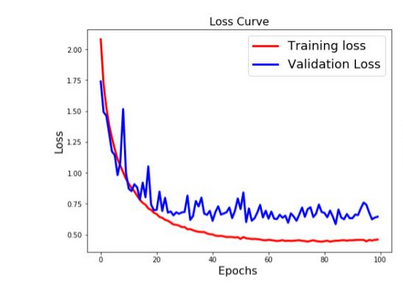
\includegraphics[scale=0.4]{./tex/regularisation/earlystop.png}\\

    On observe que la courbe d'erreur d'apprentissage est comparable à un logarithme inversé. Sur cet exemple, le sur-apprentissage ne semble pas présent.
    \caption{Exemple de courbe d'erreur d'apprentissage et de validation}
    \label{earlystop}
\end{figure}

\subsection{Data Augmentation}

Une des difficultés principales des réseaux de neurones est l'exigence d'une quantité importante de données d'apprentissage, quantité qui augmente avec la profondeur du réseau. Il n'est pas rare d'utiliser des jeux d'apprentissage contenant des millions voire des milliards d'entités, notamment dans l'étude du langage (Natural language Processing). \\

\noindent Obtenir un jeu de données est difficile, chronophage (et potentiellement cher si il doit être annoté dans le cas du traitement du langage ou de la segmentation d'image). Il est donc indispensable d'utiliser des méthodes afin, à partir d'une entité, d'en créer d'autres de manière artificielle. Il est possible de créer tout type de données de manière artificielle à partir d'une base suffisante le permettant (texte, signal 1D, 2D, ...). Chaque type de données utilise des méthodes différentes propres à son type. \\

\noindent Ainsi, dans le cas d'une image (signal 2D), plusieurs approches sont possibles:
\begin{itemize}
    \item \textbf{Variation géométrique}: Rotation, inversion, symétrie, translation
    \item \textbf{Analyse de densité de la distribution de pixels (via l'histogramme)}: contraste, filtrage, effet flou
    \item \textbf{Analyse statistiques}: Création par PCA, Création par ZCA
    \item \textbf{Signal bruité}: Ajout de bruit gaussien, bruit poivre et sel, bruit multiplicatif
    \item \textbf{Création de contenu}: Création de patterns génériques (fusionner deux photos par "collage" brut par exemple - efficace dans le cadre de la segmentation)
\end{itemize}

\noindent Il existe de nombreuses autres méthodes et ce, pour tout type de données. Un jeu d'apprentissage est de qualité si il est le plus représentatif et diversifié possible. Cette étape est donc importante car un jeu de données de qualité est une \textbf{condition nécessaire et primordiale} pour un apprentissage de qualité. \textbf{Peu importe la qualité du modèle, si les données sont de médiocre qualité, l'apprentissage sera mauvais}.

\subsection{Complexité de l'architecture et mémoire}
\label{deepcompsec}
Le Deep Learning a connu un regain de popularité grâce à l'évolution matérielle qui, dorénavant, supporte ce type d'architecture. Néanmoins, les réseaux très profonds demandent des ressources très importantes qui ne sont pas à la portée de tous (particulier comme professionnel). Un modèle complexe demande un temps très important d'apprentissage et le temps de prédiction peut être trop important pour supporter les conditions du temps réel (analyse vidéo ou vocale par exemple). De plus, une contrainte importante de mémoire dédiée peut avoir lieu dans le cadre de structures limitées telle que l'embarqué. Il est donc important de proposer des approches pour optimiser l'architecture d'un réseau. En effet, il est \textbf{important} de ne pas associer la profondeur d'un réseau avec une preuve de qualité. Un réseau très profond peut être moins performant qu'un réseau plus simple bien que sa capacité d'abstraction soit plus forte. Les difficultés d'apprentissage sont un facteur déterminant et il est souvent plus aisé d'optimiser un réseau plus petit qu'affronter la complexité d'un modèle théoriquement plus performant mais plus délicat à développer.\\

\noindent Pour cela, différentes méthodes de simplification de modèle existe, notamment \textit{Deep Compression}\cite{deepcomp_deep}. Cette méthode reprend l'idée de suppression des poids faibles issue du \textit{Dense-Sparse-Dense training}. L'objectif de cette compression est de limiter le temps d'apprentissage du modèle (de ce fait, sa complexité) et la mémoire nécessaire pour le stocker. L'approche \textit{Sparse} limite la complexité du modèle et l'optimisation de la mémoire est réalisée en deux étapes. Nous ne détaillerons pas ces deux étapes en détails, pour cela, veuillez vous référer au papier associé. \textit{Deep Compression} se déroule ainsi:

\begin{enumerate}
    \item \textbf{Sparse}: Suppression des poids faibles du réseau
    \item \textbf{Optimisation des poids et des gradients}: Afin de limiter le stockage de valeurs, une approche par clustering (Kmeans) est réalisée afin de réaliser des clusters de poids semblables. Ces poids seront donc, dans un premier temps, représentés par la valeur du centroïde\footnote{L'initialisation du Kmeans est une étape importante à étudier et à ne pas négliger} du cluster (souvent associé au barycentre). Les matrices du réseau seront donc associées à des index pointant sur la valeur du centroïde concerné. Les gradients de chacun des poids sont calculés, additionnés entre eux selon la répartition de leurs poids associés parmi les clusters définis précédemment et les gradients de chaque cluster multipliés par le pas d'apprentissage. La valeur des centroïdes sera alors mise à jour par la soustraction de la valeur du centroïde avec celle du gradient du cluster associé.
    \item \textbf{Application du codage de Huffman}: Afin de limiter le poids des matrices de poids (ou d'index), on applique un codage de Huffman. le codage de Huffman permet de réaliser une compression de données sans perte.
\end{enumerate}

\noindent Un exemple illustratif de la phase 2 est visible sur la Figure \ref{deepcomp}. Il existe d'autres méthodes bien que ce genre d'approche soit, aujourd'hui encore, expérimental et peu appliqué dans l'industrie. Cependant, il est fort probable qu'elles se développeront dans le futur du fait de la complexité grandissante des modèles crées.

\begin{figure}
    \centering
    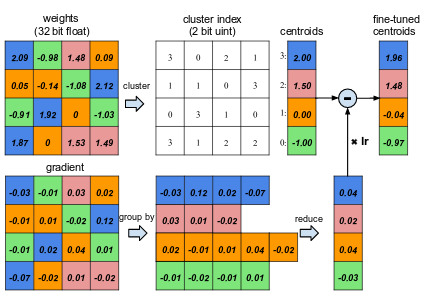
\includegraphics[scale=0.4]{./tex/regularisation/deepcomp.png}
    \caption{Optimisation réalisée sur les matrices de poids par Deep Compression}
    \label{deepcomp}
\end{figure}

\subsection{Transfer Learning}
\textbf{Important}: Cette partie va supposer que vous avez une connaissance générale des \textbf{réseaux convolutifs}. Si non, veuillez vous référer à la Section \ref{conv_sec}. On supposera le cas d'un réseau convolutif pour illustrer cette partie.\\

\noindent L'une des grandes problématiques du Deep learning est son temps d'apprentissage. Même sur des modèles jugés simples, l'apprentissage demande des ressources matérielles importantes et ce, pour une longue durée. L'objectif du \textit{Transfer Learning} est d'étudier les capacités d'un apprentissage à se généraliser à différents problèmes. Par exemple, un réseau convolutif ayant appris sur un jeu de d'images spécifiques peut-il être réutilisé sur un autre jeu d'images ? Si oui, dans quelle mesure ? Cette problématique est l'un des sujets de recherche parmi les plus actifs avec des retombés applicatives très importantes. Cette fonctionnalité est très importante dans le cas d'analyse d'image ou de texte (projection vectorielle de mots ou Words Embeddings)\\

\noindent Dans le cadre du Deep Learning, l'ensemble des approches de Transfer Learning sont exploitées. Chaque approche possède ses propres familles de réseaux et spécificités.

\paragraph{Inductive Transfer - Parameter Transfer}

\noindent La méthode \textit{Parameter Transfer} est particulièrement populaire, notamment pour les réseaux convolutifs. La problématique sous-jacente à cette approche revient à définir si des poids d'un réseau peuvent être utilisés par un autre réseau pour son apprentissage. \\

\noindent Classiquement, les couches de convolution d'un réseaux convolutifs peuvent être interprétées comme des extracteurs d'attributs d'une image, i.e extraire l'information utile et discriminante. Ces attributs sont alors différenciables par un réseau Feed-Forward standard. Il est évident que le modèle Feed-Forward est entraîné à discriminer les entités selon le jeu de données d'apprentissage. Il n'est pas pas ou très peu ré-utilisable dans d'autres contextes\footnote{Un réseau qui a appris à discriminer un chat ne pourra discriminer une voiture}. Mais il est logique de se demander si extraire des attributs d'une image est généralisable ou spécialisé d'un jeu de données particulier.\\

\noindent Les couches de convolution agissent comme des couches d'abstraction de l'image. Les premières couches isolent grossièrement les attributs de l'image et les couches finales, analysent ces attributs de manière plus spécifique et détaillée. Ainsi, plus le modèle est profond, plus sa représentation finale des données aura un haut niveau d'abstraction spécifique aux données d'apprentissage et ses couches finales seront très affiliées au données d'apprentissage (couches généralistes $\underset{\infty}{\longrightarrow}$ couches spécialisées). Les couches de convolution peuvent ainsi être généralisées car l'extraction d'attribut d'une image n'est pas nécessairement associée à une catégorie de données spécifiques (notamment dans les premières couches de convolution) car très généralistes.\\

\noindent Pour illustrer, supposons que nous souhaitons différencier deux voitures. Tout d'abord, nous considérerons la taille, la couleur dominante par exemple, i.e le comportement des premières couches de convolution alors que par la suite, nous étudierons la forme des jantes ou des rétroviseurs. Analyser la taille et la couleur peut être utile pour discriminer deux chats mais analyser la forme des jantes est peu efficace... Ainsi, le \textit{Transfer Learning} permet de limiter le "gaspillage" d'apprentissage mais des précautions doivent être prises selon les spécificités du modèle qu'on souhaite réutiliser et les nouvelles données d'apprentissage.\\

\noindent Aujourd'hui, il existe des jeux de données variées et de grande qualité (ImageNet, Cifar,...). Ces jeux de données sont très diversifiées (avec des centaines voire des milliers de classes). Ils sont donc généralistes\footnote{Si on cherche à étudier des entités d'un même domaine d'activité. Etudier des images de microbiologie à partir d'un modèle ayant appris sur des images issues d'expériences en astrophysique sera difficile quelque soit la diversité de l'apprentissage sur son domaine.}. De nombreux modèles pré-entraînés sur ces données sont en open-source et facilitent grandement le temps d'apprentissage.\\

\noindent Trois possibilités s'offrent à l'utilisateur:
\begin{enumerate}
    \item \textbf{Extracteur figé}: Dans cette configuration, on juge que les couches exportées sont fiables et finalisées. On figera donc leurs poids en bloquant les modifications par rétropropagation. Dans le cas d'une extraction de couches de convolution, la sortie obtenue par ces couches est appelée \textbf{CNN codes}.

    \item \textbf{Extracteur variable}: Dans cette configuration, les couches exportées ne sont pas figées et continuent d'apprendre durant la spécialisation du réseau sur le nouveau jeu de données. Le \textit{Transfer learning} agit donc comme une initialisation des poids du réseau (bien plus pertinent que l'aléatoire).

    \item \textbf{Modèle pré-entrainé}: Bien qu'il y ait des modèles puissants réalisés (en général) par des universités et/ou des entreprises privées, une communauté importante s'est développée pour favoriser la création de modèles déjà pré-entrainés. Ces modèles sont souvent moins "performants" que les modèles réputés et reconnus du fait de la différence de ressources et de temps d'apprentissage du réseau. Néanmoins, il est possible de trouver des réseaux ayant appris sur un jeu de données plus semblables au votre que les modèles standards ayant appris sur des données généralistes. Ces modèles offrent donc une alternative très performante notamment dans le cadre de l'initialisation de poids. On parlera alors de \textit{Fine-Tuning}.

\end{enumerate}
\noindent Le choix de l'approche à choisir dépend essentiellement de la taille du nouveau jeu de données et de leurs différences.
\begin{itemize}
    \item \textbf{Nouveau jeu de données similaire au jeu d'apprentissage et de petite taille}: A cause de la petite taille du nouveau jeu de données, le risque de sur-apprentissage est important. Comme le jeu de données d'apprentissage et proche du nouveau jeu de données, il est préférable de figer les couches de convolution et d'apprendre uniquement un nouveau modèle Feed-Forward pour la classification.

    \item \textbf{Nouveau jeu de données similaire au jeu d'apprentissage et de grande taille}: Grâce à la grande taille du jeu de données, il est possible de mettre à jour les poids des couches transférées car le risque de sur-apprentissage est plus faible. Le Transfer Learning joue un rôle d'initialisation des poids dans cette configuration et l'apprentissage spécialisera votre modèle.

    \item \textbf{Nouveau jeu de données de petite taille et très différent du jeu d'apprentissage}: Cette situation est peu  propice au Transfer Learning. En effet, le jeu d'apprentissage de petite taille ne permet pas un apprentissage des poids performant, il est donc nécessaire de limiter la mise à jour des poids des couches transférées. Cependant, la différence importante entre les deux jeux de données présente un risque de mauvaise performance due à la sur-spécialisation de ces couches. Afin de trouver un compromis, il est intéressant de ne pas garder \textbf{l'intégralité} des couches de convolutions mais d'en garder un sous-ensemble en supprimant les dernières couches qui présentent la spécialisation la plus forte. Ainsi, nous transférons que les couches les plus généralistes qu'on peut supposer performantes pour différencier des images de catégories différentes. Bien sûr, un nouveau modèle Feed-Forward doit être appris intégralement.

    \item \textbf{Nouveau jeu de données différent du jeu d'apprentissage et de grande taille}: Dans cette configuration, la grande taille du jeu de données permet un apprentissage. Néanmoins, la différence entre les deux jeux posent problème quant à la quantité des couches à transférer. Il est souvent préférable, grâce à la capacité d'apprentissage du nouveau jeu de données, d'utiliser un réseau pré-entrainé (autres que les modèles standards) qui a appris sur des données comparable aux votres afin d'initialiser les poids et d'utiliser vos données pour le spécialiser en mettant à jour les couches transférées. Un nouveau modèle Feed-Forward doit être appris.
\end{itemize}

\noindent \textbf{Important}: Le modèle Feed-Forward n'est pas impératif. En effet, d'autres algorithmes d'apprentissage automatique peuvent être utilisés notamment le SVM ou le XGboost. Néanmoins, les réseaux de neurones présentent une bonne efficacité et permettent une implémentation plus aisée en permettant la réalisation d'un modèle qui limite les dépendances de concepts.\\

\noindent Il est très difficile de considérer l'ensemble des caractéristiques d'un phénomène, c'est pourquoi la capacité de généralisation d'un modèle de \textit{Machine Learning} est très importante. Il n'est pas capital de représenter l'intégralité des hypothèses possibles\footnote{C'est d'ailleurs un travail irréalisable} mais il est nécessaire de survoler l'ensemble des grandes possibilités de représentation. Plus ce travail de diversité sera fait, plus le jeu de données sera de qualité. Il est donc évident qu'un jeu de données de grande taille aura tendance à être de meilleure qualité. Néanmoins, ce n'est pas une condition suffisante !

\paragraph{Transductive Transfer - Domain Adaptation - A FAIRE}
%https://arxiv.org/pdf/1802.03601.pdf
\subsection{Réseaux de neurones et méthodes d'Ensemble - A FAIRE}
\subsubsection{Bagging - A FAIRE}
%http://cs231n.github.io/neural-networks-3/#ensemble
\subsubsection{Boosting - A FAIRE}
